\documentclass[tikz,border=10pt]{standalone}
\usepackage{tikz}
\usetikzlibrary{shapes.geometric, arrows.meta, positioning, automata}

\begin{document}
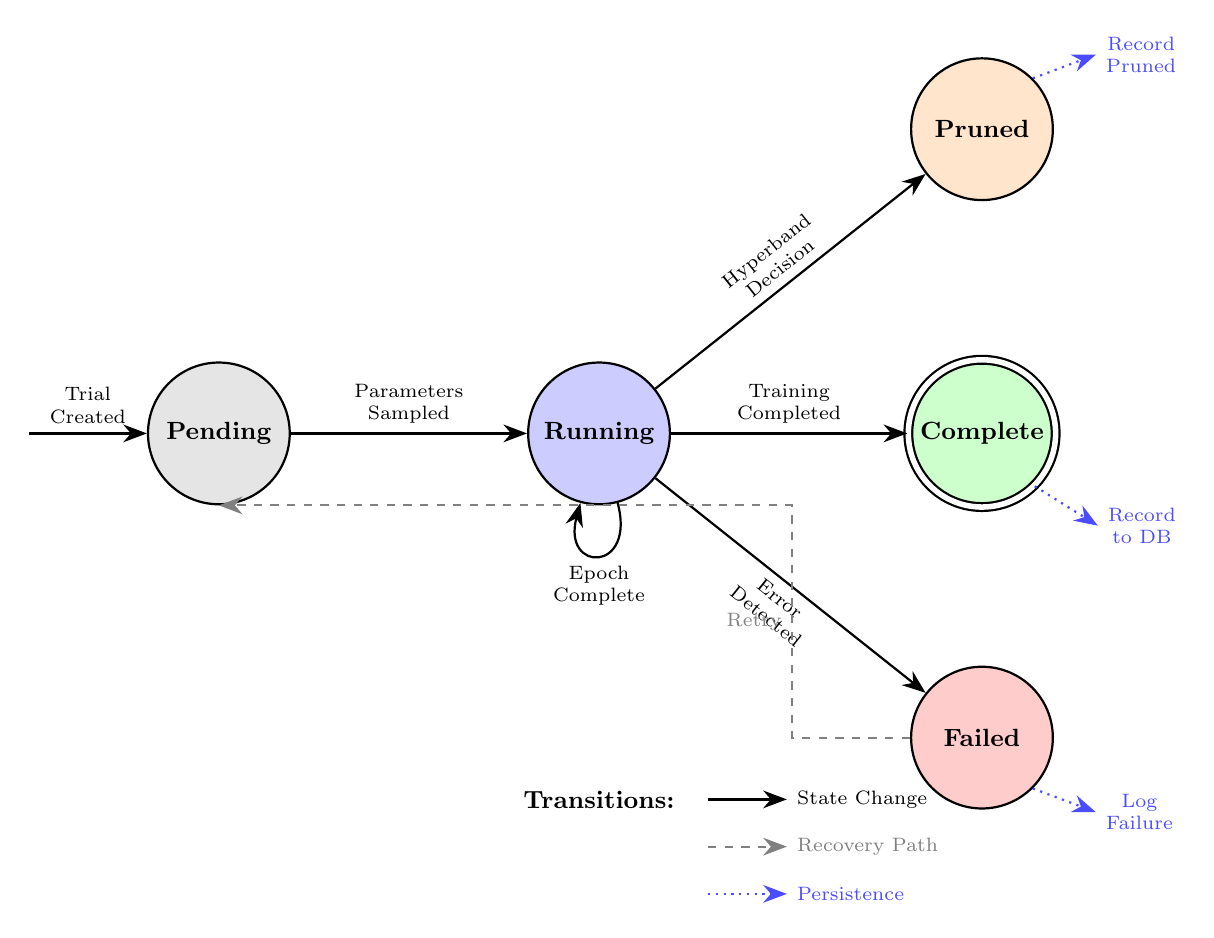
\begin{tikzpicture}[
    node distance=2.5cm and 3cm,
    state/.style={circle, draw=black, thick, minimum size=1.8cm, align=center, font=\small\bfseries},
    initial/.style={state, fill=gray!20},
    running/.style={state, fill=blue!20},
    terminal/.style={state, fill=green!20, double, double distance=2pt},
    failed/.style={state, fill=red!20},
    pruned/.style={state, fill=orange!20},
    arrow/.style={-{Stealth[length=3mm]}, thick},
    label/.style={font=\scriptsize, align=center}
]

% States
\node[initial] (init) {Pending};
\node[running, right=of init] (running) {Running};
\node[terminal, right=of running] (complete) {Complete};
\node[failed, below=2cm of complete] (failed) {Failed};
\node[pruned, above=2cm of complete] (pruned) {Pruned};

% Initial arrow
\draw[arrow] ([xshift=-1.5cm]init.west) -- (init.west) node[midway, above, label] {Trial\\Created};

% Transitions
\draw[arrow] (init) -- (running) node[midway, above, label] {Parameters\\Sampled};

\draw[arrow] (running) -- (complete) node[midway, above, label] {Training\\Completed};

\draw[arrow] (running) -- (pruned) node[midway, above, sloped, label] {Hyperband\\Decision};

\draw[arrow] (running) -- (failed) node[midway, below, sloped, label] {Error\\Detected};

% Self-loops for running state
\draw[arrow] (running) to[loop below, looseness=5] node[below, label] {Epoch\\Complete} (running);

% Recovery paths (dashed)
\draw[arrow, dashed, gray] (failed.west) -- ++(-1.5,0) |- node[pos=0.25, left, label, color=gray] {Retry} (init.south);

% Database persistence arrows
\draw[arrow, dotted, blue!70] (complete.south east) -- ++(0.8,-0.5) node[right, label, color=blue!70] {Record\\to DB};
\draw[arrow, dotted, blue!70] (failed.south east) -- ++(0.8,-0.3) node[right, label, color=blue!70] {Log\\Failure};
\draw[arrow, dotted, blue!70] (pruned.north east) -- ++(0.8,0.3) node[right, label, color=blue!70] {Record\\Pruned};

% Legend
\node[below=3.5cm of running, font=\small\bfseries] (legend) {Transitions:};
\node[right=0.3cm of legend] (leg1) {};
\draw[arrow] (leg1.west) -- ++(1,0) node[right, font=\scriptsize] {State Change};
\draw[arrow, dashed, gray] ([yshift=-0.6cm]leg1.west) -- ++(1,0) node[right, font=\scriptsize] {Recovery Path};
\draw[arrow, dotted, blue!70] ([yshift=-1.2cm]leg1.west) -- ++(1,0) node[right, font=\scriptsize] {Persistence};

\end{tikzpicture}
\end{document}
